\documentclass[conference]{IEEEtran}
\IEEEoverridecommandlockouts
\usepackage{cite}
\usepackage{amsmath,amssymb,amsfonts}
\usepackage{algorithmic}
\usepackage{graphicx}
\usepackage{textcomp}
\usepackage{xcolor}
\usepackage{booktabs}
\usepackage{url}
\usepackage{hyperref}

\def\BibTeX{{\rm B\kern-.05em{\sc i\kern-.025em b}\kern-.08em
    T\kern-.1667em\lower.7ex\hbox{E}\kern-.125emX}}

\begin{document}

\title{Design and Implementation of SentinelAgent: An AI-Assisted Framework for Cybersecurity Incident Investigation and Human-Approved Response Simulation}

\author{
\IEEEauthorblockN{Pranav Mahesh Palled, Pranay Pandurang Patil, Omkar Gurav, and Mayur Narayan Dharwadkar}
\IEEEauthorblockA{\textit{Department of Computer Science and Engineering} \\
\textit{KLS Gogte Institute of Technology}\\
Belagavi, Karnataka, India \\
Email: \{24u0237, 24u0274, 24u0309, 24u0027\}@students.git.edu}
}

\maketitle

\begin{abstract}
Modern Security Operations Centers (SOCs) face heavy alert fatigue, high false-positive rates, and lengthy incident triage workflows. While Large Language Models (LLMs) and automated response systems offer potential efficiency gains, giving unconstrained AI agents direct control over production infrastructure introduces severe risks of hallucinated evidence, prompt injection exploits, and accidental network outages. This paper presents SentinelAgent, an AI-assisted cybersecurity platform that integrates threat detection, forensic investigation, and human-authorized simulated response. SentinelAgent combines 1-minute sliding-window heuristic rules with an unsupervised Isolation Forest model with 100 estimators to detect anomalous authentication attempts from streaming SSH logs. When an incident is flagged, an autonomous two-phase LLM investigation agent queries read-only database tools within a strict 5-round ceiling. An in-memory provenance registry (AuthorizedProvenanceSet) records retrieved database identifiers and validates citations in the generated report, rejecting uncollected references. To ensure operational safety, response actions require Two-Person Integrity, preventing operators from approving their own proposals. Approved containment actions execute strictly within a persistent PostgreSQL simulation ledger with zero live operating system or firewall modifications, followed by synthetic probe verification, database state integrity constraints, and trigger-enforced PostgreSQL audit logging. We packaged SentinelAgent as a multi-tier container deployment across six unprivileged services and five Docker networks, comprising three internal and two external bridge networks. Our evaluation verified 197 deployment regression tests, 126 agent and memory unit tests, 4 frontend security invariants, and a local Docker deployment rehearsal on Docker Engine 29.9.2. A tracked-file secret scan reported no credential findings.
\end{abstract}

\begin{IEEEkeywords}
Cybersecurity, Incident Detection, Artificial Intelligence, Incident Investigation, MITRE ATT\&CK, Human-in-the-Loop, Response Orchestration, Security Automation.
\end{IEEEkeywords}

\section{Introduction}
Modern enterprise networks and cloud computing infrastructures generate massive streams of security audit logs and authentication telemetry daily. Security Operations Centers (SOCs) are tasked with continuously monitoring these telemetry streams, identifying anomalous behaviors, investigating Indicators of Compromise (IOCs), and enacting rapid mitigation strategies \cite{nelson2025incident}. However, security analysts face severe alert fatigue caused by high false-positive ratios, fragmented contextual data, and repetitive manual correlation procedures, as documented in operational SOC literature \cite{chhetri2024towards}.

To alleviate analyst workload, organizations increasingly explore Security Orchestration, Automation, and Response (SOAR) frameworks alongside generative artificial intelligence and Large Language Models (LLMs) \cite{islam2019multivocal}. Despite their natural language reasoning and analytical synthesis capabilities, deploying autonomous AI agents directly into live production networks introduces critical operational and security risks:
\begin{enumerate}
    \item \textbf{Hallucination and Fabricated Evidence:} LLMs can generate plausible-sounding but factually unsupported assertions, inventing network entities, IP addresses, or adversarial techniques not grounded in underlying telemetry.
    \item \textbf{Indirect Prompt Injection:} Malicious inputs embedded in security audit logs or retrieved historical incident records can manipulate agent instruction streams, corrupting investigative outputs \cite{greshake2023not}.
    \item \textbf{Unverified Autonomous Disruptions:} Autonomous response actions executed directly on live firewalls or software-defined networking switches without deterministic verification can inadvertently block legitimate business traffic, sever administrative access, and induce severe self-inflicted outages.
\end{enumerate}

To address these challenges, we designed and implemented \textbf{SentinelAgent}, an AI-assisted cybersecurity platform that integrates threat detection, forensic investigation, and human-authorized simulated response into a unified workflow. SentinelAgent was developed to provide SOC analysts with structured, evidence-backed investigative support while keeping all response decisions strictly under human oversight.

The system combines statistical anomaly detection with rule-based heuristics to identify suspicious SSH authentication events. For each flagged incident, an AI agent running Google Gemini inspects database evidence through constrained, read-only tools. To mitigate ungrounded citations and defend against prompt injection attempts within telemetry, every piece of evidence cited in confirmed findings is validated against an in-memory provenance registry before a report is finalized. When containment is recommended, the platform requires two distinct operators to propose and approve the action. To avoid operational disruption to live networks, approved actions are executed inside a persistent database simulation ledger rather than live firewall infrastructure, followed by synthetic verification probes and tamper-resistant audit logging.

The principal engineering contributions of this work include:
\begin{enumerate}
    \item \textbf{Dual Threat Detection Pipeline:} Integration of heuristic sliding-window rules and unsupervised Isolation Forest anomaly detection (100 estimators) over streaming authentication events, coupled with automated 5-minute incident correlation.
    \item \textbf{Provenance Validation Barrier:} An in-memory provenance registry (\textit{AuthorizedProvenanceSet}) that tracks canonical database query citations and excludes historical memory from confirmed citations, causing report generation to fail closed if uncollected references appear.
    \item \textbf{Server-Authoritative ATT\&CK Alignment:} Deterministic server-side mapping of observed behavioral patterns against the MITRE ATT\&CK Enterprise Matrix (v20.1: 15 tactics, 227 techniques, 479 sub-techniques) \cite{mitre2026attack, strom2018mitre}, enforcing explicit disclosures when telemetry bounds prevent conclusive sub-technique assertion.
    \item \textbf{Two-Person Integrity Approval Gate:} Dual-authorization enforcement modeled after dynamic separation of duty \cite{saltzer1975protection, ahn2000role}, application-enforced to prohibit an analyst from self-approving their own mitigation proposals.
    \item \textbf{Simulation-Only Execution and Verification:} Response execution restricted strictly to a persistent PostgreSQL simulation ledger with zero live operating system or firewall modifications, followed by synthetic probe verification, database state integrity constraints, and trigger-enforced PostgreSQL audit logging.
    \item \textbf{Hardened Multi-Network Container Topology:} A Docker Compose deployment isolating six unprivileged services across five networks (three internal, two external bridge) with non-root execution and zero-DELETE PostgreSQL runtime permissions.
\end{enumerate}

\section{Related Work}
Incident detection, investigation, and response have evolved significantly from manual rule inspection to automated orchestration and AI-assisted analysis.

\subsection{Threat and Brute-Force Detection}
SSH and authentication services remain prime targets for automated credential attacks \cite{najafabadi2015detection}. Traditional intrusion detection systems (IDS) rely heavily on static signature rules, which struggle to detect slow, distributed password guessing or low-and-slow campaigns. Vinayakumar et al. \cite{vinayakumar2019deep} demonstrated deep learning approaches for intelligent intrusion detection, showing high detection rates over complex traffic representations. However, high-capacity deep learning models require extensive labeled training datasets and introduce non-trivial inference latencies. Liu et al. \cite{liu2008isolation} introduced the Isolation Forest algorithm, an efficient, unsupervised ensemble method that detects anomalies by isolating outliers using random decision trees without calculating distance or density metrics. SentinelAgent adopts Isolation Forest in conjunction with sliding-window heuristic rules to provide responsive, dual-engine threat detection.

\subsection{Security Orchestration and Human-in-the-Loop Operations}
To address the overwhelming volume of security telemetry, Security Orchestration, Automation, and Response (SOAR) platforms have gained widespread adoption \cite{islam2019multivocal}. Bartwal et al. \cite{bartwal2022security} explored automated SOAR engines for deploying honeypots, emphasizing the value of structured automated workflows. Nonetheless, full response automation carries substantial risk: erroneous or hallucinated blocklist updates can sever critical administrative links or take production services offline. Saltzer and Schroeder \cite{saltzer1975protection} established the foundational security principle of Separation of Privilege, asserting that critical operations should require dual authorization. Ahn and Sandhu \cite{ahn2000role} and Bertino et al. \cite{bertino1999specification} formalized dynamic Separation of Duty (DSoD) constraints in workflow access control models, while Jha et al. \cite{jha2008towards} demonstrated the necessity of formally verifying policy enforcement rules. SentinelAgent incorporates these access control principles into response orchestration, ensuring that no containment action can execute without two distinct human operators.

\subsection{LLMs in SOCs and Prompt Injection Defense}
The advent of generative AI has spurred research into deploying LLMs as interactive SOC analyst assistants \cite{chhetri2024towards}. While Retrieval-Augmented Generation (RAG) frameworks \cite{lewis2020retrieval} enable LLMs to query external knowledge bases, Greshake et al. \cite{greshake2023not} demonstrated that LLMs integrated with external data repositories are vulnerable to indirect prompt injection. Attackers can embed adversarial instructions inside log files or historical cases to manipulate the agent's investigative trajectory. SentinelAgent addresses these risks through structured defense-in-depth: recalled historical memories are quarantined as untrusted contextual data, structural JSON escaping mitigates instruction breakout, and server-side citation validation aborts report assembly if uncollected identifiers are referenced.

\section{System Architecture and Methodology}
SentinelAgent operates as an integrated incident investigation and response workflow comprising eleven operational stages, as illustrated in Fig. 1 and Fig. 2.

\begin{figure*}[t]
\centering
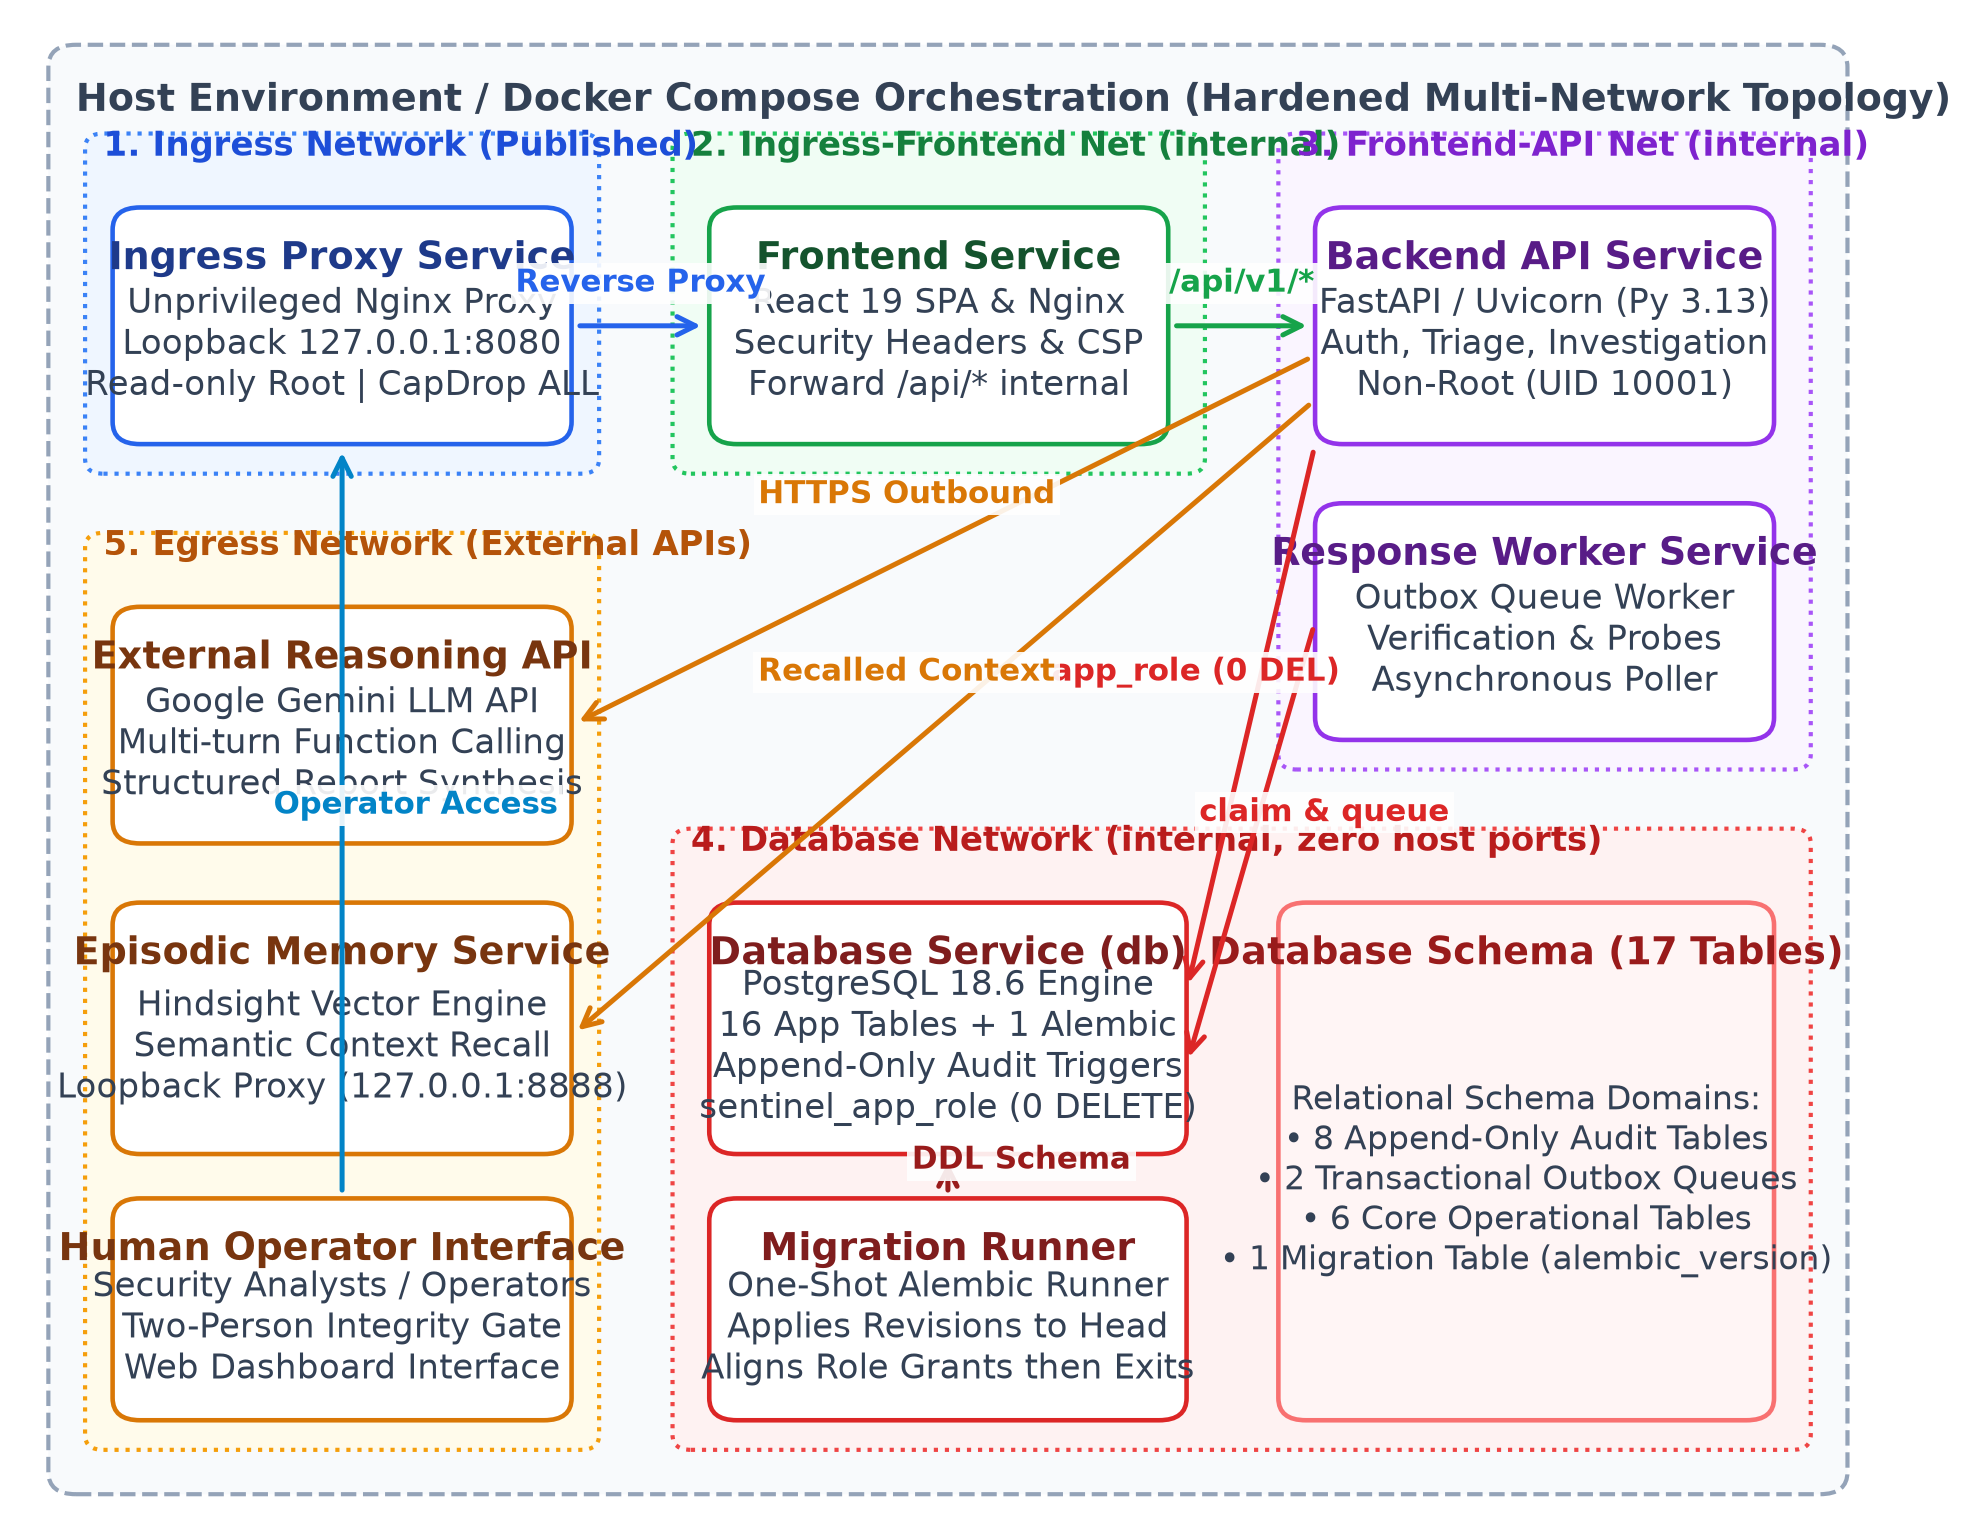
\includegraphics[width=0.92\textwidth]{figures/fig1_system_architecture.png}
\caption{SentinelAgent overall system architecture illustrating the multi-network container topology, six unprivileged services, relational storage domains (16 application tables + 1 Alembic migration record), and isolation boundaries.}
\label{fig:arch}
\end{figure*}

\subsection{Stage 1: Telemetry Ingestion and Feature Extraction}
We generated synthetic SSH authentication events using the event structure implemented in SentinelAgent. For testing, source IP addresses were selected from the TEST-NET ranges reserved for documentation under RFC 5737 \cite{arkko2010ipv4}. The events were submitted through the application's SSH ingestion endpoint (\texttt{POST /api/v1/events/ssh}). Each event records an \texttt{event\_id} (UUID), \texttt{event\_timestamp} (UTC), \texttt{source\_ip} (INET), \texttt{username}, \texttt{authentication\_result} (\texttt{success} or \texttt{failure}), and \texttt{event\_type} (\texttt{failed\_password}, \texttt{accepted\_password}, etc.).

The \texttt{FeatureExtractor} service aggregates raw events into fixed 1-minute UTC sliding windows grouped by source IP. For each temporal window, it extracts six typed behavioral features:
\begin{enumerate}
    \item $N_{\text{total}}$: Total authentication attempts.
    \item $N_{\text{failed}}$: Count of failed attempts.
    \item $N_{\text{success}}$: Count of successful logins.
    \item $N_{\text{users}}$: Distinct usernames targeted.
    \item $R_{\text{fail}}$: Failure ratio ($N_{\text{failed}} / N_{\text{total}}$).
    \item $F_{\text{susp}}$: Boolean flag indicating suspicious success (a successful login immediately preceded by $\ge 5$ failures within the window).
\end{enumerate}

\subsection{Stage 2: Dual-Engine Threat Detection}
The feature vector is dispatched concurrently to two detection engines:
\begin{itemize}
    \item \textbf{Rule-Based Engine (\texttt{RuleDetector}):} Evaluates deterministic threshold signatures:
    \begin{align}
        \text{Rule R001} &: N_{\text{failed}} > 10 \quad (\text{SSH Brute Force Burst}) \\
        \text{Rule R002} &: F_{\text{susp}} = \text{True} \quad (\text{Success After Failures})
    \end{align}
    \item \textbf{Machine Learning Engine (\texttt{IsolationForestDetector}):} An unsupervised ensemble of 100 isolation estimators ($n_{\text{estimators}}=100$, random state 42) trained on baseline normal feature vectors. The detector computes an anomaly normality score $s(\mathbf{x})$. To establish an anomaly decision boundary, the threshold is calibrated at the 5th percentile of normality scores on normal baseline samples using the configuration parameter \texttt{default\_target\_fpr = 0.05} (a quantile target rather than an experimentally measured false-positive rate), flagging windows falling below this score as behavioral anomalies.
\end{itemize}

\subsection{Stage 3: Incident Creation and Correlation}
The \texttt{DetectionOrchestrator} evaluates detections emitted by either engine. When an anomaly is detected, it correlates the event against active, open incidents from the same source IP within a 5-minute temporal window. If an open incident exists, the detection result is appended; otherwise, a new \texttt{Incident} is instantiated with \texttt{status='open'}, \texttt{response\_status='not\_proposed'}, and initial severity set to \texttt{NULL} to prevent premature unverified severity scoring prior to investigation.

\subsection{Stage 4: Investigation Lifecycle Coordination}
The \texttt{InvestigationService} coordinates the investigation lifecycle. State transitions proceed deterministically from \texttt{pending} to \texttt{in\_progress}, culminating in \texttt{completed} or \texttt{failed}. To guarantee deadlock-free execution under concurrent workloads, the service enforces a strict hierarchical database lock acquisition order:
\begin{equation}
\text{Incident} \longrightarrow \text{Investigation} \longrightarrow \text{ToolRun}
\end{equation}
Abandoned or crashed investigation tasks are automatically reclaimed using atomic \texttt{SKIP LOCKED} batch queries, ensuring system liveness without manual intervention.

\subsection{Stage 5: Autonomous Investigation Agent}
Forensic investigation is driven by the \texttt{InvestigationAgent}, which operates across two distinct, isolated phases:
\begin{itemize}
    \item \textbf{Phase A (Tool Exploration Loop):} The agent interacts with a set of strictly bounded, server-side read-only tools: \texttt{get\_ssh\_events}, \texttt{get\_incident\_details}, \texttt{search\_by\_username}, and \texttt{get\_prior\_evidence}. The loop is strictly constrained to a maximum ceiling of five interaction rounds ($\text{MAX\_TOOL\_ROUNDS} = 5$). Tools execute with zero mutation privileges.
    \item \textbf{Phase B (Structured Synthesis):} All analytical tools are disabled. The agent synthesizes its investigative conclusions into a Pydantic-validated \texttt{InvestigationReport} conforming to a rigid JSON schema defining executive summaries, confirmed findings, and indicator relationships.
\end{itemize}

\begin{figure*}[t]
\centering
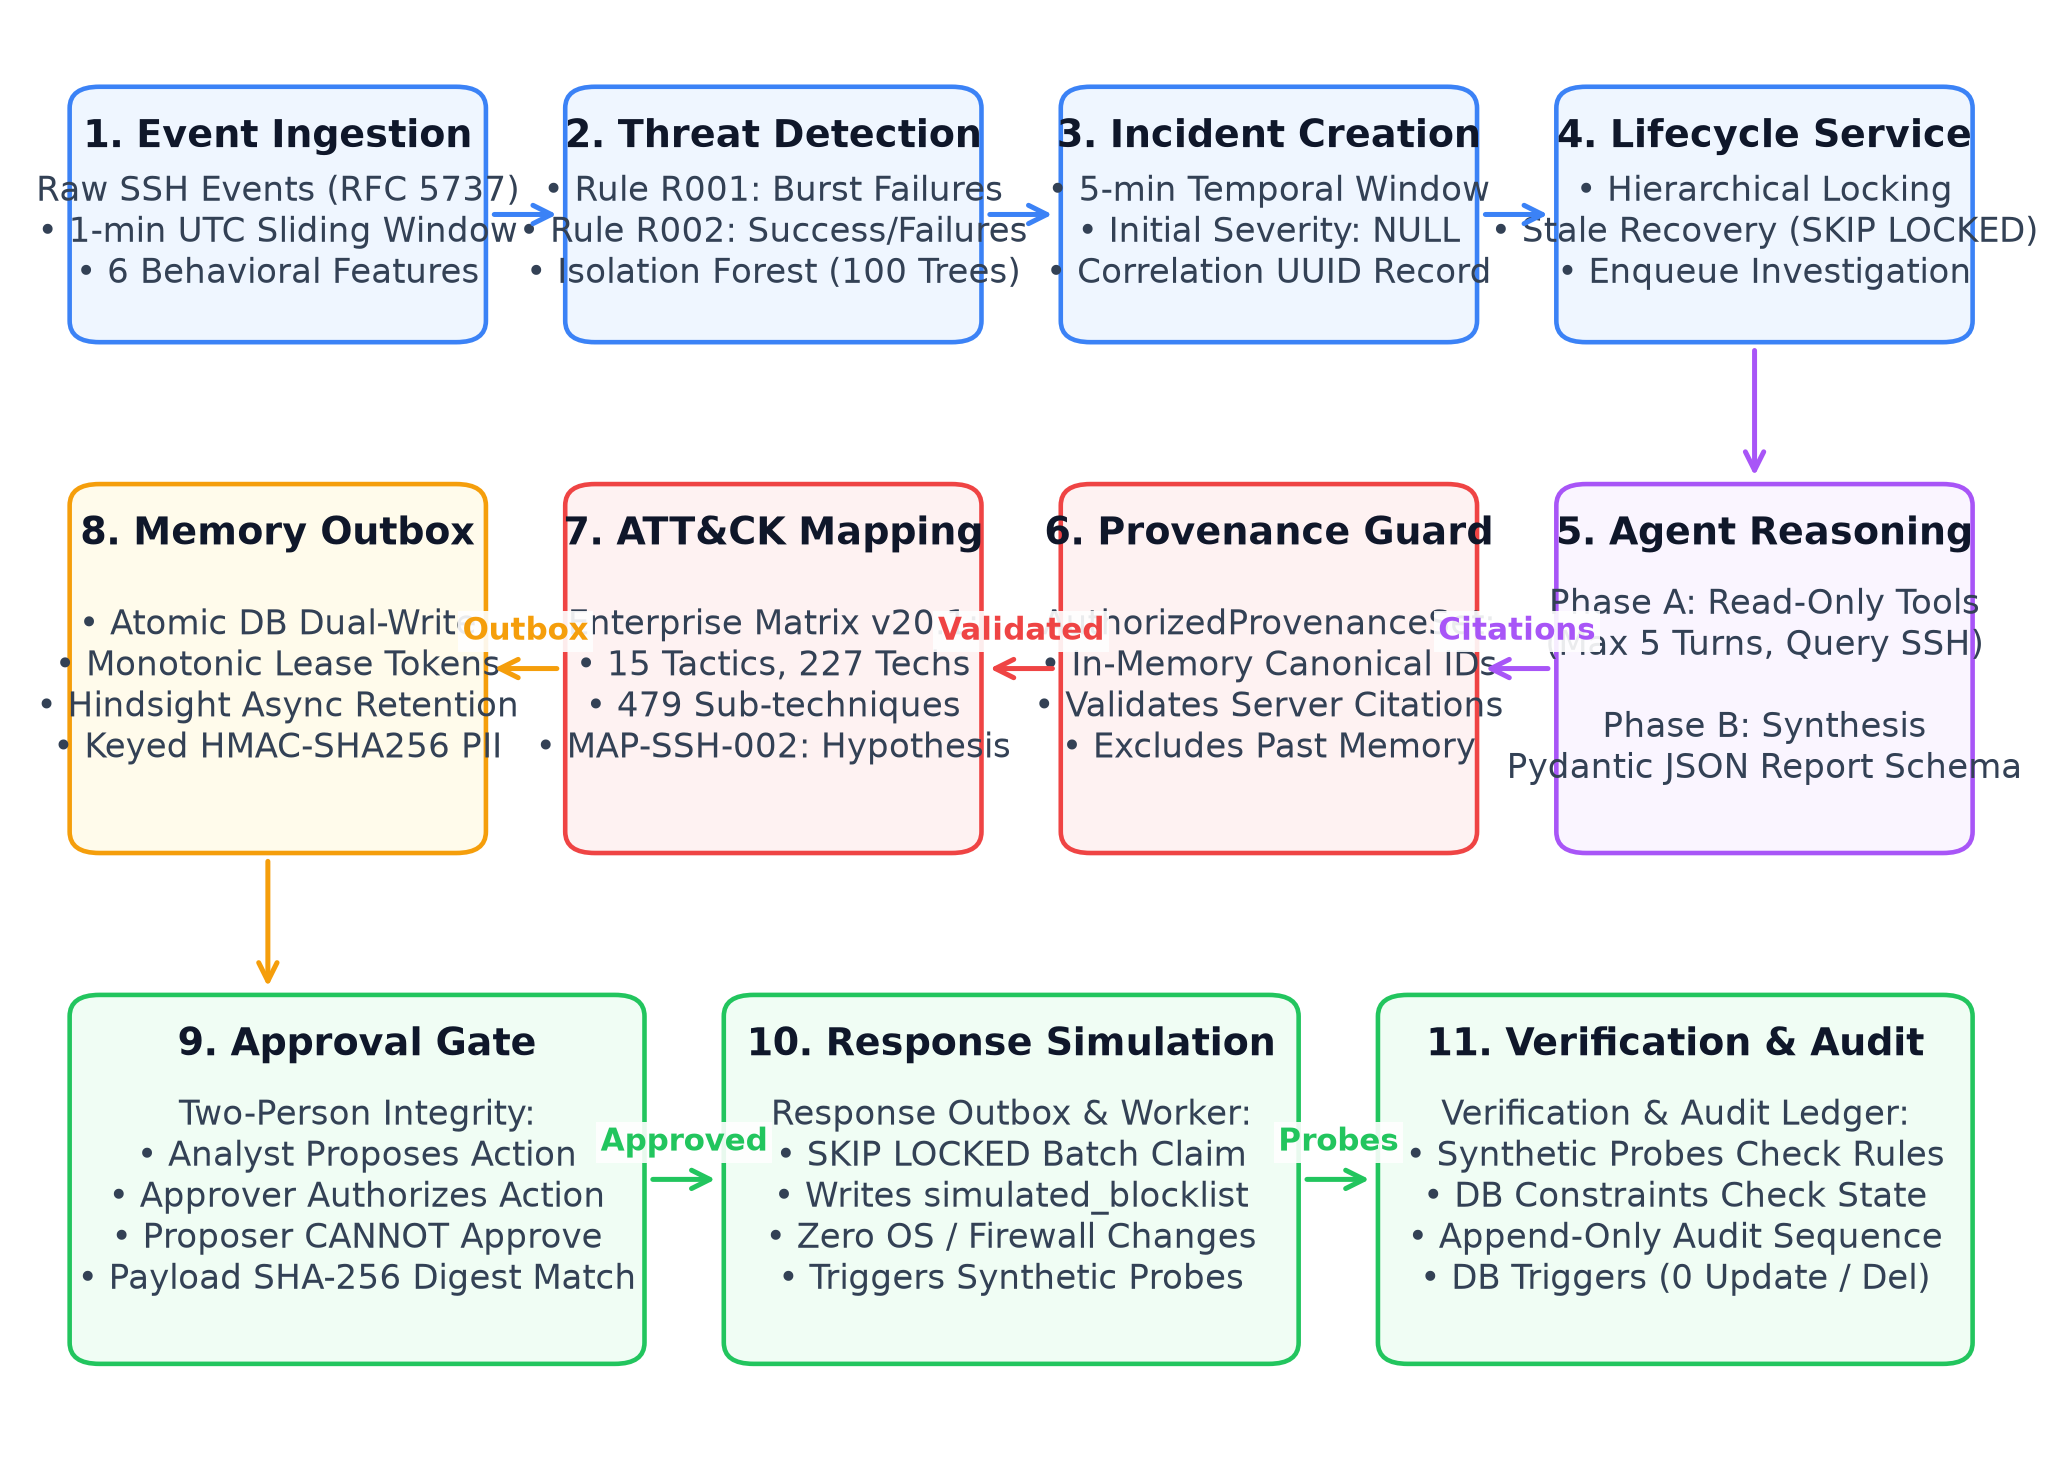
\includegraphics[width=0.92\textwidth]{figures/fig2_workflow.png}
\caption{End-to-end incident detection, forensic investigation, and response simulation workflow illustrating the eleven operational stages, provenance tracking, and human approval gates.}
\label{fig:workflow}
\end{figure*}

\subsection{Stage 6: Provenance Validation Barrier}
To mitigate LLM hallucinations and defend against prompt injection from adversarial audit logs, SentinelAgent introduces the \textit{AuthorizedProvenanceSet}. During Phase A, every entity retrieved through server-side tools is registered in an in-memory Python set using canonical, typed identifiers (e.g., \texttt{ssh\_events/<uuid>}, \texttt{evidence\_items/<uuid>}).

During report finalization, the completion service verifies every citation referenced in the agent's confirmed findings against the \textit{AuthorizedProvenanceSet}. If the agent references an uncollected entity, an external URL, or a forged identifier, the transaction immediately aborts with a \texttt{ProvenanceValidationError}, discarding the report. The registry validates citations against records retrieved through approved server-side tools; it does not guarantee that all natural-language statements generated by the LLM are inherently true.

\subsection{Stage 7: Server-Authoritative MITRE ATT\&CK Mapping}
Adversary tactics and techniques are mapped through the deterministic \texttt{MitreMappingEngine} against authoritative MITRE ATT\&CK Enterprise Matrix definitions (v20.1, comprising 15 tactics, 227 techniques, and 479 sub-techniques) \cite{mitre2026attack, strom2018mitre}. Three mapping rules are evaluated:
\begin{itemize}
    \item \texttt{MAP-SSH-001} (Brute Force, \texttt{T1110}): Evaluates vertical failure density against a single account within a 15-minute window.
    \item \texttt{MAP-SSH-002} (Password Spraying, \texttt{T1110.003}): Evaluates horizontal failure distribution across $\ge 5$ distinct accounts within a 30-minute window with $\le 3$ failures per account.
    \item \texttt{MAP-SSH-003} (Long-Horizon Brute Force, \texttt{T1110}): Evaluates low-frequency login attempts requiring continuous 2-hour telemetry coverage.
\end{itemize}

Crucially, SentinelAgent enforces explicit telemetry limitation disclosures: because standard SSH audit logs do not capture plaintext attempted passwords, \texttt{MAP-SSH-002} deterministically restricts its classification to \texttt{mapping\_status = HYPOTHESIS} with \texttt{confidence = MEDIUM}, attaching a mandatory disclosure that password reuse cannot be conclusively verified from telemetry alone. AI suggestions are never treated automatically as confirmed evidence without server-side validation.

\subsection{Stage 8: Transactional Memory Outbox and Historical Context}
To facilitate long-term institutional knowledge retention without impacting investigative throughput, SentinelAgent implements the Transactional Outbox pattern \cite{richardson2018microservices}. When an investigation completes, its memory document payload is written to the \texttt{incident\_memory\_outbox} table within the exact same PostgreSQL database transaction as the investigation completion.

An asynchronous in-process worker (\texttt{HindsightMemoryOutboxWorker}) claims outbox entries using PostgreSQL transaction-level advisory locks:
\begin{equation}
\texttt{pg\_advisory\_xact\_lock}(\texttt{hashtext}(bank\_id), \texttt{hashtext}(doc\_id))
\end{equation}
A monotonic lease token fencing counter prevents stale workers from writing uncoordinated state. Sensitive identifiers (IPs, usernames) are pseudonymized into deterministic 128-bit HMAC-SHA256 digests (\texttt{ip:v1:<hex32>}) before dispatch to the companion Hindsight vector memory engine. When historical memories are recalled in future investigations, they are quarantined within an untrusted prompt block (\texttt{TRUSTED\_HISTORICAL\_INSTRUCTIONS}), explicitly excluded from the \textit{AuthorizedProvenanceSet}, and treated only as untrusted contextual information.

\subsection{Stage 9: Two-Person Integrity Approval Gate}
Following investigation, mitigation actions are proposed via \texttt{POST /api/v1/incidents/\{id\}/response/proposals}. SentinelAgent implements strict Two-Person Integrity modeled on dynamic Separation of Duty \cite{ahn2000role}. The proposal defines the target IP, justification, expiration deadline, and computes a SHA-256 digest over the canonical JSON payload:
\begin{equation}
H_{\text{payload}} = \text{SHA-256}(\text{CanonicalJSON}(\text{payload}))
\end{equation}

When an approver authorizes the proposal via \texttt{POST /api/v1/response/actions/\{id\}/approve}, the application service enforces three mandatory validation checks:
\begin{enumerate}
    \item \textbf{Separation of Actors:} $\text{Operator}_{\text{approver}} \neq \text{Operator}_{\text{proposer}}$. Self-approval is rejected at the API layer with HTTP 403 Forbidden.
    \item \textbf{Role Verification:} The approver must possess the authenticated role \texttt{OperatorRole.APPROVER}.
    \item \textbf{Payload Invariance:} The authorized digest must identically match the proposal digest ($H_{\text{approved}} == H_{\text{payload}}$).
\end{enumerate}

\subsection{Stage 10: Simulation-Only Response Execution}
Upon approval, the action is queued in the \texttt{response\_outbox}. The background \texttt{ResponseWorker} claims queued commands using atomic \texttt{SKIP LOCKED} semantics.

In accordance with safety-first design, SentinelAgent enforces a simulation-only response adapter: the worker commits the mitigation action strictly to the persistent PostgreSQL relational ledger table \texttt{simulated\_blocklist\_entries}. Zero operating system commands (\texttt{iptables}, \texttt{nftables}, \texttt{netsh}) or cloud firewall API calls exist in the codebase. The platform does not execute real firewall or operating system commands and does not perform actual network containment, preventing unintended host or network disruption during testing and demonstration.

\subsection{Stage 11: Synthetic Probe Verification and Tamper-Resistant Audit Trail}
Immediately following simulated execution, the verification engine generates active synthetic verification probes against the simulated rule state. The results are recorded in \texttt{verification\_reconciliation\_records} and evaluated against database check constraints that enforce valid application state:
\begin{equation}
\text{Resolution} = \text{'confirm\_verified'} \implies N_{\text{intercepted}} = N_{\text{generated}}
\end{equation}
\begin{equation}
\text{Resolution} = \text{'confirm\_failed'} \implies N_{\text{intercepted}} = 0 \land \text{Coverage} = \text{True}
\end{equation}
If probes yield inconsistent or partial telemetry, the status is set to \texttt{inconclusive}, triggering mandatory manual review by an authorized operator.

\begin{figure}[t]
\centering
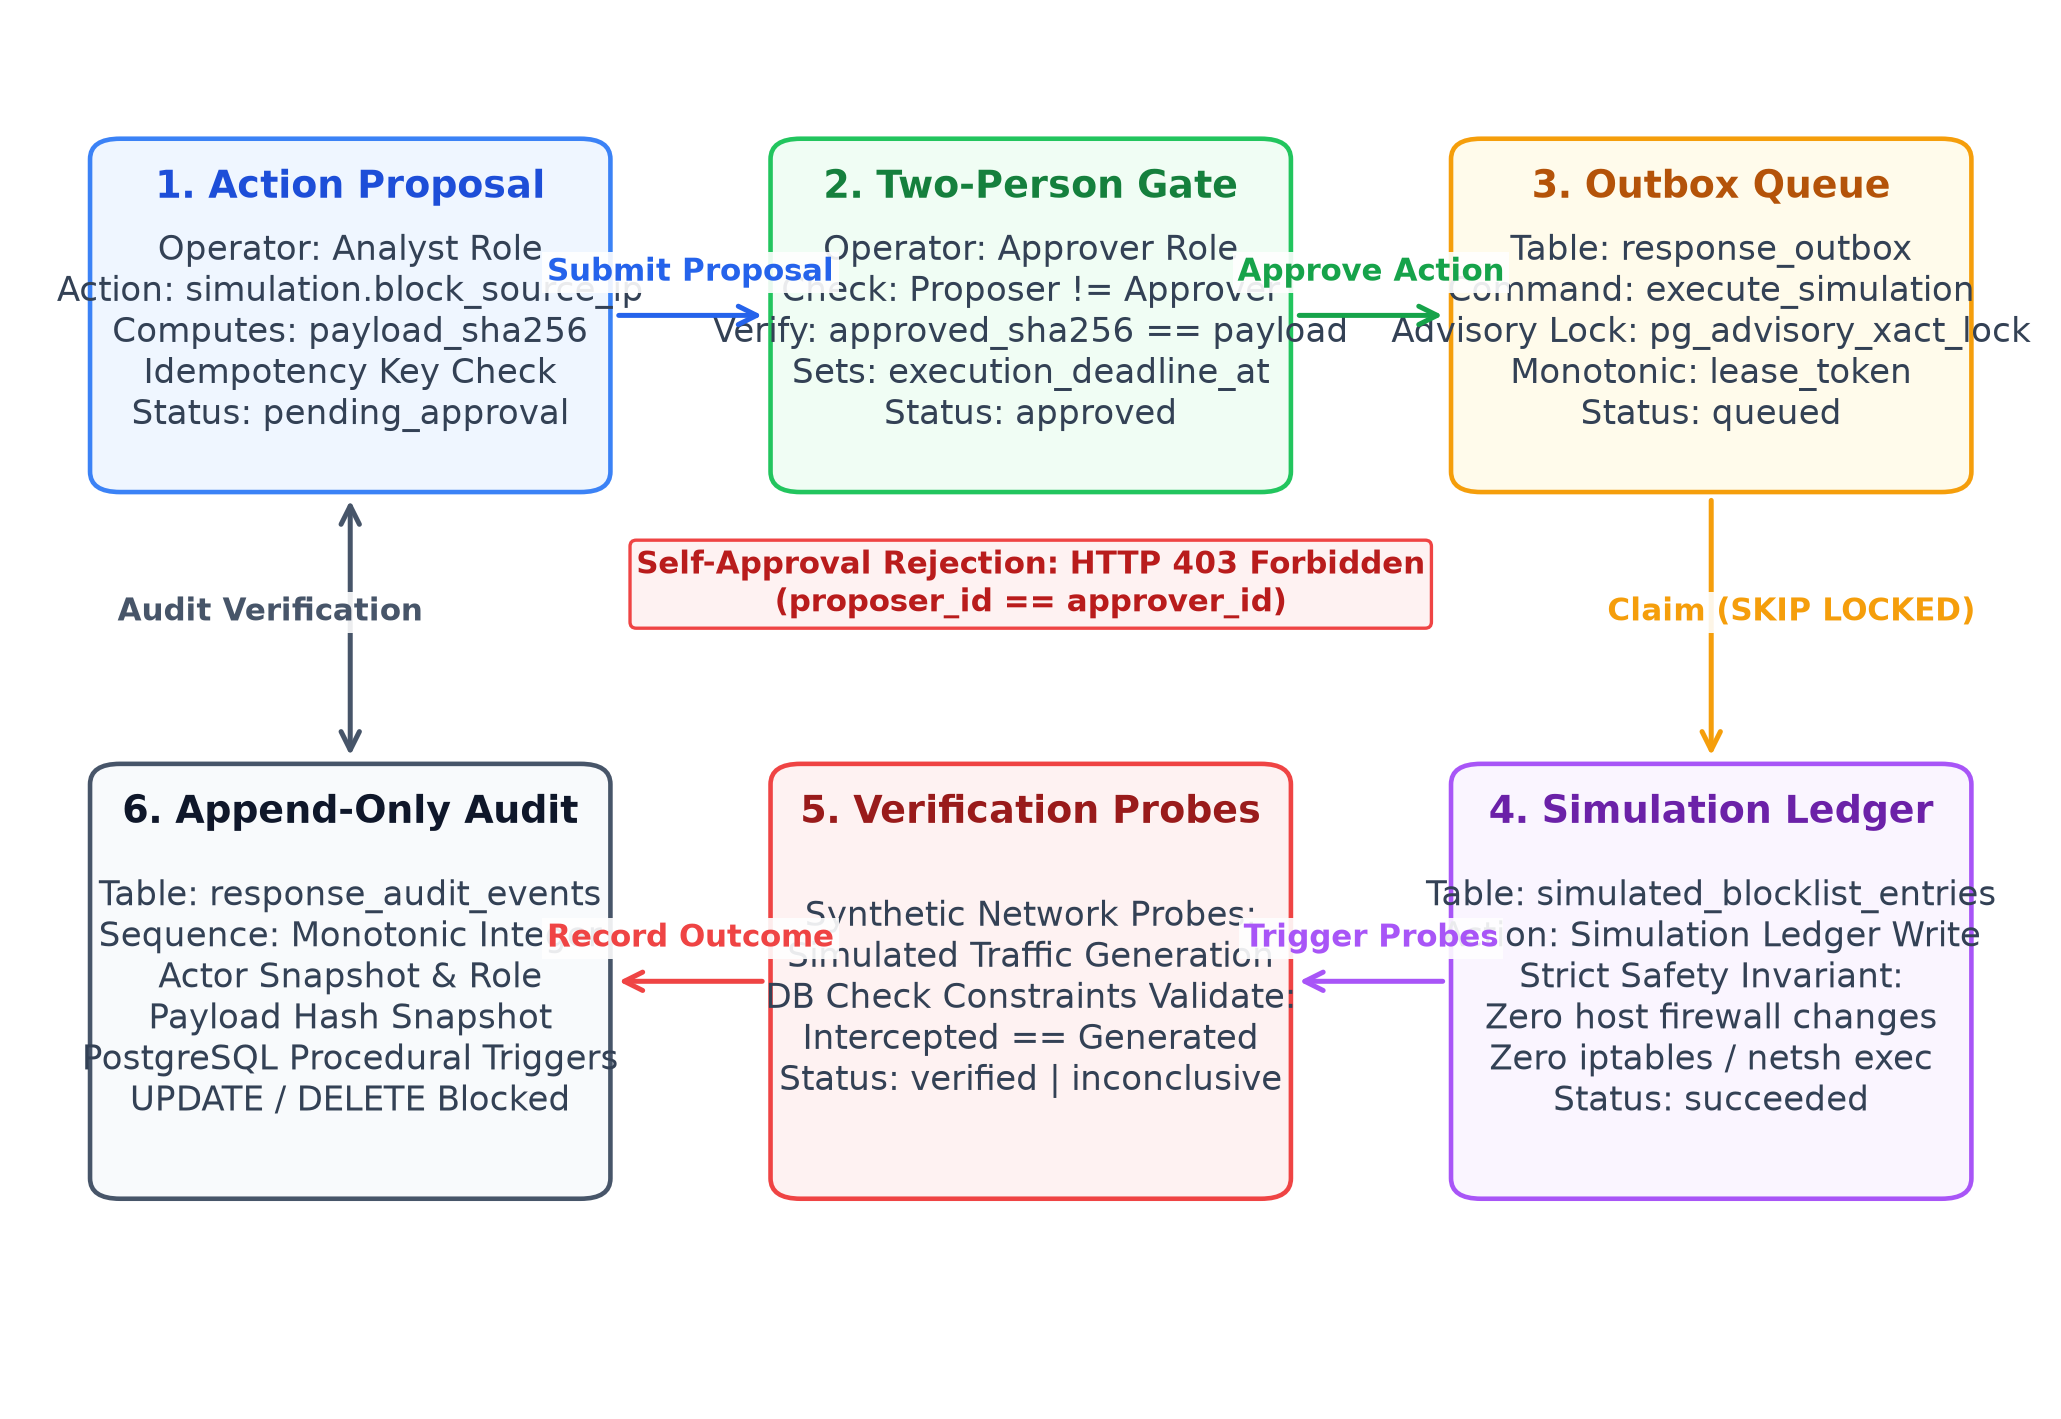
\includegraphics[width=0.48\textwidth]{figures/fig3_lifecycle.png}
\caption{Two-Person Integrity response lifecycle illustrating proposal hashing, self-approval rejection, simulation execution, and active verification.}
\label{fig:lifecycle}
\end{figure}

Every state mutation across the proposal, approval, execution, and verification phases is logged to the \texttt{response\_audit\_events} table. Each event records an incrementing sequence number, actor ID, role snapshot, client IP, payload digest, and timestamp. Immutability is enforced at the database layer via PostgreSQL procedural triggers (\texttt{fn\_prevent\_immutable\_modification()}) that intercept and abort any \texttt{UPDATE}, \texttt{DELETE}, or \texttt{TRUNCATE} statements.

\section{Implementation Details}
SentinelAgent is constructed using Python 3.13, FastAPI, SQLAlchemy 2.1.8, PostgreSQL 18.6, React 19, and Docker Compose v2 (Table I). The database schema comprises 16 application tables plus 1 Alembic migration-tracking table (17 database tables total) managed across six linear Alembic revisions terminating at head \texttt{34ea070e907d}.

\begin{table}[t]
\caption{SentinelAgent Technology Stack and Deployment Specifications}
\label{tab:tech_stack}
\centering
\begin{tabular}{lll}
\toprule
\textbf{Subsystem} & \textbf{Technology / Component} & \textbf{Version / Specification} \\
\midrule
Backend Runtime & Python & 3.13.6 \\
Web Framework & FastAPI & 0.162.1 \\
ASGI Server & Uvicorn & 0.54.0 \\
Database ORM & SQLAlchemy (async \& sync) & 2.1.8 \\
Database Driver & Psycopg 3 (binary) & 3.3.8 \\
Schema Migrations & Alembic & 1.20.1 (Head: \texttt{34ea070e907d}) \\
Database Engine & PostgreSQL & 18.6-alpine (16 App + 1 Alembic Tab.) \\
Frontend UI & React / TypeScript & React 19, TypeScript 5.7 \\
Frontend Bundler & Vite / Tailwind CSS & Vite 6, Tailwind 3.4 \\
Edge Ingress & Nginx (Unprivileged) & 1.30-alpine-slim (UID 101) \\
Containerization & Docker Engine / Compose & Engine 29.9.2, Compose 5.6.1 \\
Primary Reasoning & Google Gemini API & \texttt{gemini-3.5-flash-lite} \\
Auxiliary Memory & Hindsight Semantic Engine & v1.2.1 (\texttt{gemma3:4b}, BGE-Small) \\
Threat Framework & MITRE ATT\&CK Enterprise & v20.1 (15 tactics, 227 techs, 479 sub) \\
\bottomrule
\end{tabular}
\end{table}

\subsection{Database Role Least-Privilege Separation}
The relational database layer enforces strict privilege separation between deployment operations and runtime execution through two dedicated PostgreSQL roles:
\begin{itemize}
    \item \texttt{sentinel\_migration\_role}: Owns the database schema; possesses full DDL capabilities to create tables, triggers, and indices during one-shot startup migrations.
    \item \texttt{sentinel\_app\_role}: Runtime operational role used by the API backend and asynchronous response worker. It is strictly granted \texttt{SELECT}, \texttt{INSERT}, and selective \texttt{UPDATE} privileges. In accordance with non-destructive audit requirements, \texttt{sentinel\_app\_role} possesses \textbf{zero \texttt{DELETE} privileges, zero \texttt{TRUNCATE} privileges, and zero sequence manipulation grants} across all 16 application tables.
\end{itemize}

\subsection{Container Security and Network Hardening}
The deployment environment is configured as a multi-tier containerized topology defining six distinct services: \texttt{ingress}, \texttt{frontend}, \texttt{api}, \texttt{worker}, \texttt{migration}, and \texttt{db}. Security hardening parameters include:
\begin{itemize}
    \item \textbf{Non-Root Execution:} Containers execute under dedicated unprivileged users (UID 10001 for Python application services, UID 101 for Nginx proxies, UID 70 for PostgreSQL).
    \item \textbf{Capability Dropping:} All application and web services drop all Linux kernel capabilities (\texttt{cap\_drop: [ALL]}).
    \item \textbf{Read-Only Filesystems:} Web and application containers mount read-only root filesystems (\texttt{read\_only: true}) with temporary writable storage restricted to in-memory, non-executable \texttt{tmpfs} mounts (\texttt{noexec,nosuid}).
    \item \textbf{Network Isolation:} Network traffic is partitioned across five Docker networks. Three networks are declared internal (\texttt{internal: true}) and have zero external connectivity: \texttt{sentinel\_ingress\_frontend\_network}, \texttt{sentinel\_frontend\_network}, and \texttt{sentinel\_db\_network} (the database publishes zero host ports). Two networks are standard Docker bridge networks: \texttt{sentinel\_ingress\_network} (publishing the ingress proxy on loopback \texttt{127.0.0.1:8080}) and \texttt{sentinel\_egress\_network} (providing standard Layer-3 NAT outbound egress for the API and worker to dispatch HTTPS requests to external APIs). Standard Docker bridge networks do not enforce port-level egress filtering.
\end{itemize}

\section{Experimental Setup and Evaluation}
To ensure rigorous academic credibility, this evaluation reports verified test results, static security scans, and deployment rehearsals conducted against the actual SentinelAgent codebase.

\subsection{Evaluation Methodology}
The system was evaluated across four dimensions:
\begin{enumerate}
    \item \textbf{Functional Pipeline Verification:} Automated testing of event ingestion, feature extraction, rule triggering, and anomaly isolation.
    \item \textbf{Provenance Defense Testing:} Programmatic unit and integration testing of prompt injection resilience, citation verification, and PII redaction using test harness mock vectors without calling live external AI endpoints.
    \item \textbf{Two-Person Integrity and Response Safety:} Verification of application-level self-approval rejection, SHA-256 payload invariance, and simulation ledger constraints.
    \item \textbf{Hardened Deployment Rehearsal:} Multi-container initialization, migration ordering, network boundary isolation, and database volume persistence verified during a local Docker deployment rehearsal on Docker Engine 29.9.2.
\end{enumerate}

\subsection{Experimental Findings and Verified Results}
The evaluation results are summarized in Table II, Table III, and Table IV.

\begin{table}[t]
\caption{System Subsystems and Functional Responsibilities}
\label{tab:components}
\centering
\begin{tabular}{llp{4.2cm}}
\toprule
\textbf{Subsystem} & \textbf{Service Scope} & \textbf{Core Security Invariants} \\
\midrule
Detection Engine & API Service & 1-min sliding windows; dual heuristic and Isolation Forest scoring. \\
Investigation Agent & API Service & Phase A/B isolation; max 5 tool rounds; Pydantic JSON schema output. \\
Provenance Guard & API Service & \textit{AuthorizedProvenanceSet} rejects uncollected entity references. \\
ATT\&CK Mapper & API Service & Enterprise v20.1 catalog; hypothesis tagging on password spraying. \\
Two-Person Gate & API Service & Proposer ID $\neq$ Approver ID; SHA-256 payload match required. \\
Response Worker & Worker Service & Monotonic lease claiming; zero OS or firewall modifications. \\
Verification Engine & Worker Service & Synthetic probe matching; automated fallback to inconclusive. \\
Audit Ledger & Database & Immutability triggers block \texttt{UPDATE} and \texttt{DELETE} operations. \\
\bottomrule
\end{tabular}
\end{table}

\begin{table}[t]
\caption{Functional, Security, and Regression Test Results}
\label{tab:test_results}
\centering
\begin{tabular}{lccl}
\toprule
\textbf{Test Evaluation Suite} & \textbf{Tests} & \textbf{Duration} & \textbf{Evaluation Outcome} \\
\midrule
Phase 12 Deployment Security & 19 & 0.82s & 100\% Passed \\
Phase 12 Deployment Integration & 12 & 0.45s & 100\% Passed \\
Phase 12 Database Deployment & 10 & 0.61s & 100\% Passed \\
Phase 12 Role Least-Privilege & 9 & 0.38s & 100\% Passed \\
Phase 12 Config \& Secret Scoping & 147 & 3.80s & 100\% Passed \\
\midrule
\textbf{Subtotal: Deployment Regression} & \textbf{197} & \textbf{6.06s} & \textbf{100\% PASSED} \\
\midrule
Memory Serializer \& PII Redaction & 56 & 2.10s & 100\% Passed \\
Gemini Client Auth \& Formatting & 15 & 1.10s & 100\% Passed \\
Investigation Agent \& Provenance & 55 & 5.01s & 100\% Passed \\
\midrule
\textbf{Subtotal: Memory, Client \& Agent Suite} & \textbf{126} & \textbf{8.21s} & \textbf{100\% PASSED} \\
\midrule
Frontend Security \& Logic & 4 & 0.29s & 100\% Passed \\
Static Credential Scanner & 211 files & 1.20s & 0 Leaks (Code 0) \\
Database State Preservation & 47 actions & -- & 5 Demo Records Intact \\
\midrule
\textit{Complete Backend Test Inventory} & \textit{1,331} & \textit{--} & \textit{Collected (50 modules)} \\
\bottomrule
\end{tabular}
\end{table}

\begin{table}[t]
\caption{Docker Deployment Rehearsal and Isolation Matrix}
\label{tab:deployment_results}
\centering
\begin{tabular}{lllp{2.6cm}}
\toprule
\textbf{Service} & \textbf{Base Image} & \textbf{User} & \textbf{Network Attachments} \\
\midrule
\texttt{ingress} & Nginx 1.30 & UID 101 & \texttt{ingress\_net}, \texttt{ingress\_frontend} \\
\texttt{frontend} & Node 22 / Nginx & UID 101 & \texttt{ingress\_frontend}, \texttt{frontend\_net} \\
\texttt{api} & Python 3.13 & UID 10001 & \texttt{frontend\_net}, \texttt{db\_net}, \texttt{egress\_net} \\
\texttt{worker} & Python 3.13 & UID 10001 & \texttt{db\_net}, \texttt{egress\_net} \\
\texttt{migration} & Python 3.13 & UID 10001 & \texttt{db\_net} (One-shot, exited 0) \\
\texttt{db} & Postgres 18.6 & UID 70 & \texttt{db\_net} (0 host ports) \\
\bottomrule
\end{tabular}
\end{table}

As documented in Table III:
\begin{itemize}
    \item \textbf{Regression Integrity:} The 197 dedicated deployment and security regression tests passed with zero failures in 6.06 seconds.
    \item \textbf{Programmatic Provenance Defense:} In automated unit test suites (\texttt{test\_investigation\_agent.py}), 15 programmatic prompt injection test vectors embedded inside simulated telemetry records were evaluated against mock LLM responses; in all test runs, the \textit{AuthorizedProvenanceSet} rejected uncollected citations and preserved report integrity without calling external live AI APIs.
    \item \textbf{Two-Person Gate Verification:} Across multiple unit tests in \texttt{test\_auth.py} and frontend tests in \texttt{frontend.test.mjs}, attempts by an analyst to approve their own proposal consistently yielded HTTP 403 Forbidden.
    \item \textbf{Database Preservation:} Querying the local PostgreSQL instance confirmed that all 47 existing response actions and all five demonstration records remained completely intact.
    \item \textbf{Deployment Rehearsal:} The local Docker deployment rehearsal on Docker Engine 29.9.2 confirmed proper startup ordering (\texttt{db} $\to$ \texttt{migration} $\to$ \texttt{api}/\texttt{worker} $\to$ \texttt{frontend} $\to$ \texttt{ingress}), network attachment, and data persistence across project restarts.
\end{itemize}

\section{Discussion and Limitations}
Our evaluation demonstrates that combining autonomous LLM reasoning with server-side provenance boundaries and Two-Person Integrity provides structured defenses against common hazards of AI in cybersecurity: ungrounded evidence, prompt injection in telemetry, and unverified containment actions within our tested scope.

However, several engineering boundaries and limitations must be explicitly acknowledged:
\begin{enumerate}
    \item \textbf{Synthetic Telemetry Baseline:} The evaluation used synthetically generated SSH authentication events with source IP addresses drawn from the RFC 5737 TEST-NET ranges \cite{arkko2010ipv4}. Live enterprise authentication telemetry was not evaluated.
    \item \textbf{Simulation-Only Execution:} Containment actions are recorded strictly in database ledgers rather than physical firewall hardware. The system does not execute actual operating system or firewall commands and does not perform real network blocking.
    \item \textbf{Absence of Plaintext Passwords:} Because standard Linux \texttt{auth.log} telemetry excludes attempted passwords for security reasons, the platform cannot definitively prove password reuse across accounts, necessitating hypothesis classification for password spraying attacks.
    \item \textbf{Evaluation Scope:} The system has undergone local Docker deployment rehearsals; it has not yet been deployed in a public production environment. Alert fatigue reduction is an operational motivation supported by literature \cite{chhetri2024towards}, not an experimentally measured metric of this study.
\end{enumerate}

\section{Conclusion and Future Work}
This paper presented the design, implementation, and empirical verification of SentinelAgent, an AI-assisted cybersecurity platform that integrates threat detection, forensic investigation, and human-authorized response simulation. By pairing a dual-engine detection architecture with an autonomous two-phase LLM investigation agent and enforcing an in-memory provenance wall, SentinelAgent validates that reported findings correspond to server-retrieved records. Furthermore, by embedding application-enforced Two-Person Integrity, simulation-only containment within a persistent PostgreSQL ledger, active synthetic verification probes, and trigger-enforced PostgreSQL audit immutability, the platform provides a structured, auditable workflow for incident investigation while avoiding operational disruption to live network infrastructure.

Future work will focus on:
\begin{itemize}
    \item Benchmarking detection accuracy and throughput against large-scale, heterogeneous public intrusion datasets (e.g., CIC-IDS).
    \item Developing pluggable containment drivers for containerized cloud environments with automated rollback capabilities.
    \item Extending the deterministic mapping engine to cloud infrastructure and container attack matrices.
\end{itemize}

\section*{Acknowledgment}
The authors express their sincere gratitude to their project guide, Dr. Sanjeev S. Sannakki (Department of Computer Science and Engineering), for his invaluable guidance, technical insights, and constant encouragement throughout the design and implementation of SentinelAgent. The authors also gratefully acknowledge the Department of Computer Science and Engineering, KLS Gogte Institute of Technology, Belagavi, for providing computing infrastructure, laboratory facilities, and academic support.

\bibliographystyle{IEEEtran}
\bibliography{references}

\end{document}
